% 1. Introduction: Why is low power clock network important. Papers on how much energy is consumed by clock and how much can be saved
% 2. "old"-not-low power clock tree synthesis
% (3. 2D routing algorithm)
% 3. Possibilities to reduce clock power.
% 3.1 Use unbuffered trees
% 4. Clock networks for 3D stacked ICs. Different algorithms
% 4.1 Present algorithm from X. Zhang.
% 5. Conclusion

\documentclass[conference]{IEEEtran}
\IEEEoverridecommandlockouts
% The preceding line is only needed to identify funding in the first footnote. If that is unneeded, please comment it out.
\usepackage{cite}
\usepackage{amsmath,amssymb,amsfonts}
\usepackage{algorithmic}
\usepackage{graphicx}
\usepackage{textcomp}
\usepackage{caption}
\RequirePackage[utf8]{inputenc}
\def\BibTeX{{\rm B\kern-.05em{\sc i\kern-.025em b}\kern-.08em
    T\kern-.1667em\lower.7ex\hbox{E}\kern-.125emX}}
\begin{document}

\title{Low power reduction techniques for Ultra Low Power Processors}

\author{
	\IEEEauthorblockN{Karthik Sukumar}
	\IEEEauthorblockA{\textit{Department of Electrical and Computer Engineering}\\
	\textit{Technical University Munich (TUM)}\\Munich,
    Germany\\karthik.sukumar@tum.de}
}

\maketitle

\begin{abstract}
In this paper the works of J.Zhou et al. \cite{b1} and J.Tang et al. \cite{b2}
on design techniques for an ultra low-power processor is reported.

J.Zhou et al. focusses on Near-Threshold processor design for Ultra low power
processors. The paper discusses the design challenges, performance issues and solutions
of the above. The circuit level power reduction techniques are addressed here.

J.Tang et al. discusses a case study by using GPS to demonstate that an
Ultra-low power processor used along with a heavy applications processor can
lead to further power savings. The architectural level power reduction
techniques are addressed here.
\end{abstract}

\begin{IEEEkeywords}
Near-Threshold, Ultra low power, GPS, Offload Co-processor, Interrupt service
routines
\end{IEEEkeywords}

\section{Introduction} \label{sec:introduction}

Power constraint portable devices (e.g. Mobile phones, wearables, IoT
devices) require ultra low power processors in order to save battery life. Such
low power devices enable operation with the help of energy harvesters or small baterries.
Sub and Near-Threshold devices have been shown to have an overall low power
consumption and past works confirm that Near-Threshold designs are more
efficient than using clock and power gating.

For further reduction of power consumption without loss of performance we need to look at architectural
level improvements to preseve scalabililty.

\begin{figure}[htbp]
	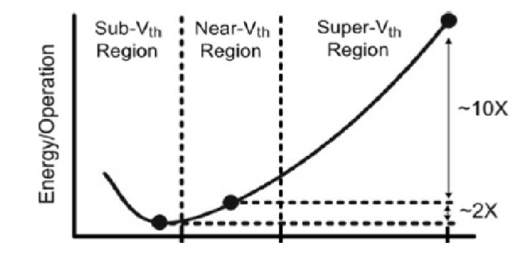
\includegraphics[width=\linewidth]{img/Pictures/Energy_comparison.png}
	\centering
	\caption{Sub/Near-Threshold operation. Source: \cite{b1}}
	\label{fig:Energy_comparison}
\end{figure}

Near-Threshold designs refer to operating the transistor slightly above the
threshold region. The major advantage of Near-Threshold over Super-Threshold operation is the decrese in energy per operation.
Dynamic energy per operation increases quadratically with voltage as ($P_{dyn}=fC_LV_{DD}^2$), where as static energy per operation increases with decreasing voltage. This is because the static power
is constant and the static energy consumption increases with increasing time period per operation (As max frequency of operation reduces with decresing supply voltage).
Hence by adding the two we get a relationship as shown in Fig. \ref{fig:Energy_comparison}. Although we see that the Sub-Threshold operation
has lower energy than the Near-Threshold, we want to find a balance between
performance and energy per operation and hence we will investigate the
functionality, variability issues and performance challenges of Near-Threshold
design in this paper.

\section{Functional Challenges of Near-Threshold Design}
\label{sec:Func_challenges}

Past research has shown that Near-Threshold design is easy to implement for ALUs and logic gates. But SRAM and level Shifter have their challenges in operating in the Near-Threshold region.

\subsection{Level Shifters}

\begin{figure}[htbp]
	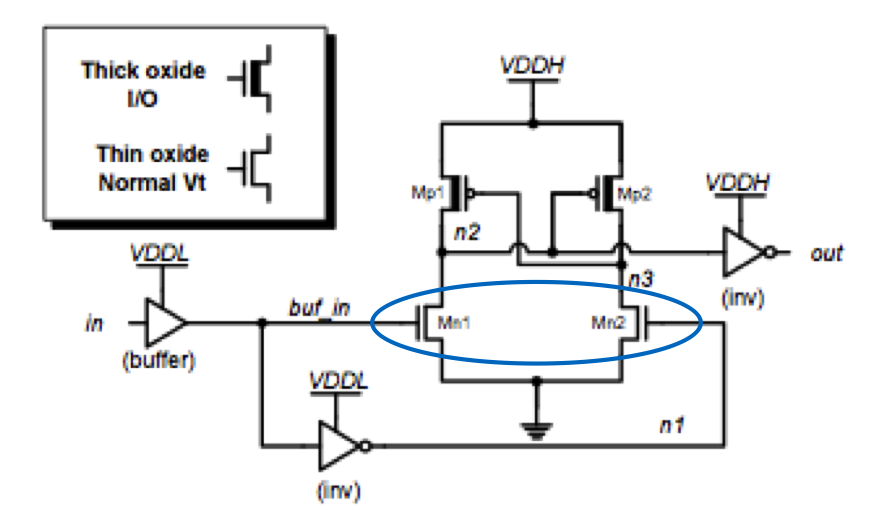
\includegraphics[width=\linewidth]{img/Pictures/Level_shift_weak.png}
	\centering
	\caption{Weak Pull ups Source: \cite{b3}}
	\label{fig:Weak_Pull_ups}
\end{figure}

In the Near-Threshold operation the pull down network as shown in the Fig. \ref{fig:Weak_Pull_ups} is weaker than the pull up network and consequently the the level shifter cant pull down to ground.

The issue of converting a Near-Threshold voltage to a super-threshold voltage
therefore needs complex circuitry which is not only low power in nature but
also scales in performance with voltage. 

\begin{figure}[htbp]
	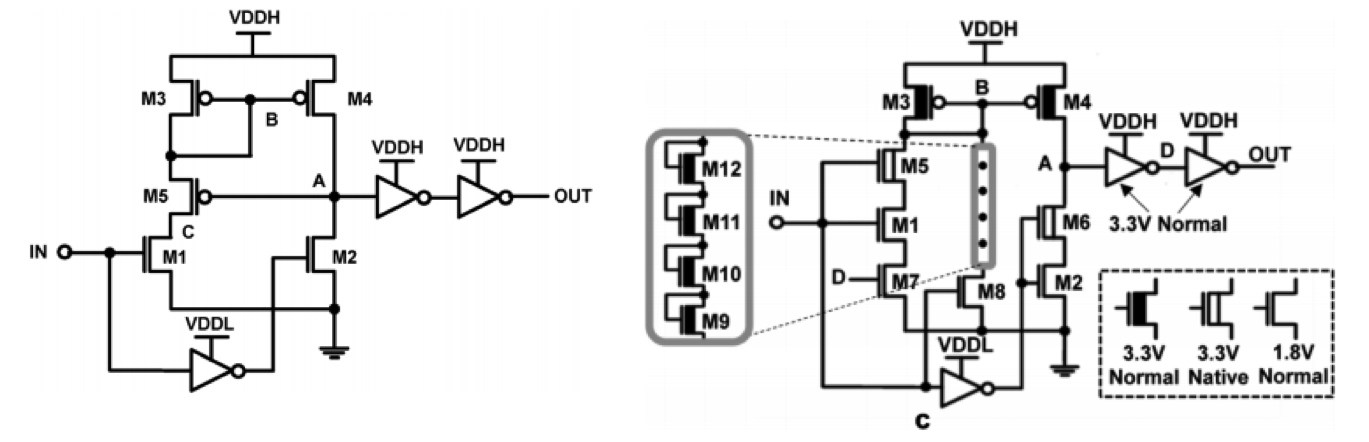
\includegraphics[width=\linewidth]{img/Pictures/Level_shifter_solution.png}
	\centering
	\caption{Weak Pull ups Source: \cite{b6}}
	\label{fig:Level_shifter_solution}
\end{figure}

In \cite{b4}\cite{b5}\cite{b6}, current mirrors based design is suggested as it provides performance scalablity
and high energy efficiency as shown in Fig. \ref{fig:Level_shifter_solution}.

\subsection{SRAM Design Challenges}
There are 2 issue with Near-Threshold SRAM design. One is that many cells share the read/write interface and the second being that the SRAM prefers small transistors for increased density. These conventions make it difficult for them to function in the Near-threshold region. Small transistors have small current driving strength and large variation at low voltages, causing read/write disturbances.

The solution to both the issues is to have a decoupled read write interface namely an 8T/10T SRAM design. Although not as dense as the traditional 6T design, they are more resistant to manufacturing variabilities.

\section{Performance Improvement for Near-Threshold Devices} \label{sec:Perf_challenges}

\subsection{Near-Threshold Device Sizing}
It has been found that the parasitic effects dominate more in the Near-Threshold than the Super-Threshold regions. Reverse Short Channel Effects (RSCE) for example is rather strong in the Near-Threshold region. As opposed to DIBL(Drain Induced Barrier Lowering) the threshold voltage decreases with increasing Channel length. Another effect is INWE(Inverse Narrow Width Effect) which causes the threshold voltage to decrease as the transistor width decreases. Minimum finger widths are therefore used to reduce delays and improve energy efficiency. By making use of the minimun-sizing method and by selectively tuning the length of critical and non-critical paths the energy efficiency can be improved while meeting the performance specification.

\subsection{Wide Dynamic Voltage Scaling}
Designing with a large voltage swing from Near/Sub-Threshold voltages to Super-Threshold voltages (e.g. from 280mV to 1.1V) enables the processors to go to deep sleep mode when not active and spull up to full power when active. This fast voltage switching is critical for energy efficiency without loss of performance.
\subsection{Parallel Processing}
The performance degradation of the Near-Threshold operation can be compensated by parallel processing. In \cite{b8}, 4 homogeneous parallel processing engines have neen designed to accelerate Near-Threshold JPEG encoding, achieving 40MB/s (or VGA, 30 fps) and a 1.33pJ/cycle at 0.6V in a 65nm process.

\section{Manufacturing Variabilty Challenges} \label{sec:Variablity}
Manfacturing variabilty plays vital part as it leads to large performance variations. As the current has an exponential relationship to voltage around the Threshold voltage, small variation in voltage can result in a large current. Therfore process variation can cause a significant variablity in delay or performance. Some of the ways mentioned below can mitigate such risks.
\subsection{Library Pruning}
Its important to characterise the standard cells at low voltage, this way the one with large performance variations and poor performance are taken out e.g: Gates with 4 stacked transistors.
\subsection{Pipeline Optimization}
Optimising pipeline depth has shown to decrease processor variabilty. It has been found that large logic depths reduce variabilties through the averaging effect. Therefore shallow pipelines with larger logic depth are adopted as a measure against process variations. As shown in Fig. \ref{fig:PplstageVSlogicdepth} the 2-stage pipeline with 75 logic gates per stage reduces the standard deviation by 19\% compared to design with 10 gates per pipeline stage.

\begin{figure}[htbp]
	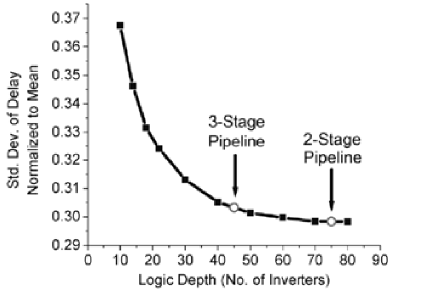
\includegraphics[width=\linewidth]{img/Pictures/PplstageVSlogicdepth.png}
	\centering
	\caption{Random variation vs number of pipeline stages \cite{b1}}
	\label{fig:PplstageVSlogicdepth}
\end{figure}

\section{Architectural Level Power Reduction Techniques} \label{sec:Case_Study}
For high performance embedded devices we need to consider architectural design
changes to maintain the performance. The Application Processor(AP) is the most
power consuming component in the design. In order to reduce the power consumption as
much as possible we need to wake up the AP only when its absolutely necessary.
Given that the peak workload on most mobile embedded devices is often
periodic interrupts or user requests we can utilise this to offload the
AP of servicing these routines.

This is illustrated with the help of a case study to show the advantages of
using an Ultra Low Power Offload Co-processor(OCP), which could be one of the
processors incorporating all the circuit level design techniques described in the earlier sections.

\subsection{Case Study: GPS}

GPS is chosen for our case study as it usually samples at 1Hz and is a periodic
event. Research has shown that GPS can consume upto 95\% of the total power
consumption of the mobile device \cite{b7}.

The system we are considering here is a typical ARM11 micro-processor which is
commonly found in most mobile phones these days. In the power profile for the AP shown in Fig. \ref{fig:Power_profile_ARM11} the CPU is initially in sleep mode
consuming 20mW before the interrupt occurs. The interrupt is serviced in 2ms (at
1000mW) and the AP dosent transition to sleep mode immediately, instead it must operate
at a lower frequency consuming 650mW for 100ms. It drops into yet another mode at
400mW for another 100ms. Only after executing in all these intermediate modes
does the CPU go back into deep sleep. Therefore although the interrupt only
takes 2ms to execute the application processor remains active for over 200ms
consuming 60mJ of energy.

\begin{figure}[htbp]
	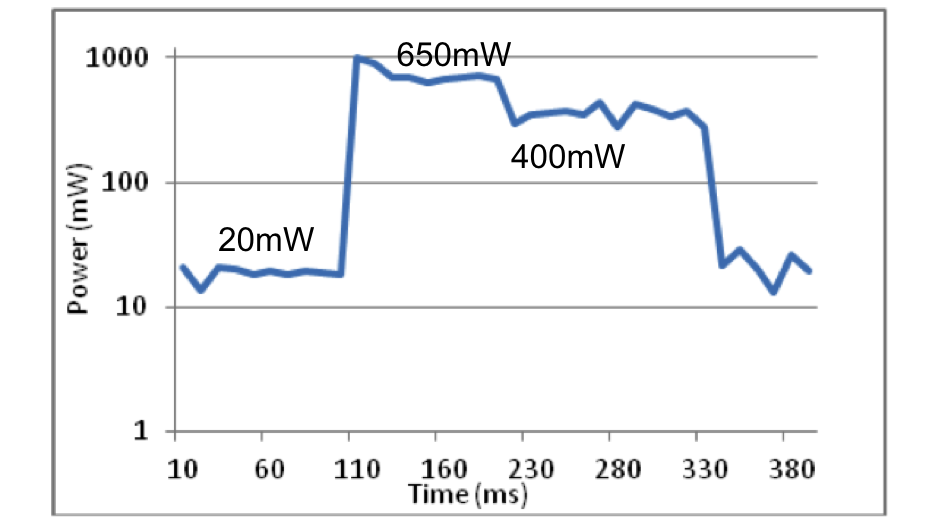
\includegraphics[width=\linewidth]{img/Pictures/Power_profile_ARM11.png}
	\centering
    \caption{Power Profile when a GPS interrupt occurs for an ARM11 CPU: \cite{b2}}
    \label{fig:Power_profile_ARM11}
\end{figure}

\section{OCP Design}
An alternative SoC design with a OCP is shown in Fig. \ref{fig:AP}. In our case study the Application Processor is an ARM11 CPU and the OCP is a MIPS32 4KS.

\begin{figure}[htbp]
	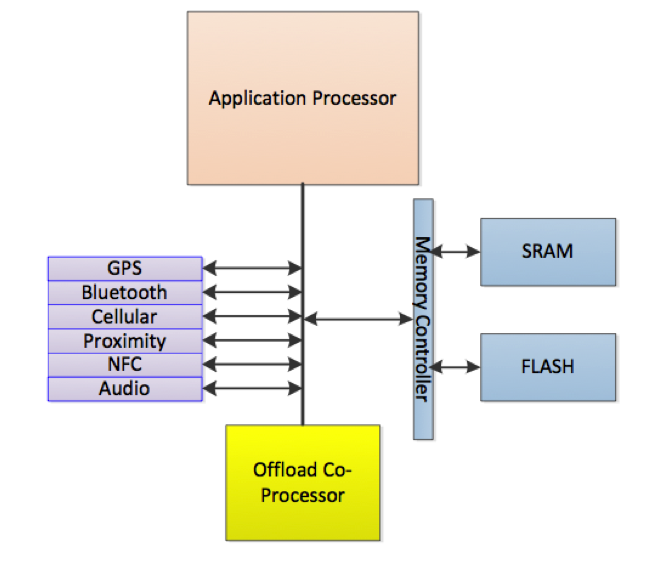
\includegraphics[width=\linewidth]{img/Pictures/AP.png}
	\centering
    \caption{SoC Design with Offload Co-Processor(OCP): \cite{b2}}
    \label{fig:AP}
\end{figure}

\subsection{Energy Analysis}

We assume a 1500mAh battery at 3.7V. The values of different modes of both the processors are shown in Table. \ref{tab:powercons}. The $P_{AP-active}$ is derived by 60mJ/200ms, which is 300mW.

\begin{center}
\captionof{table}{Power Consumption of different modes} \label{tab:powercons}
\begin{tabular}{ |l|c| } 
\hline
\textbf{Item} & \textbf{Power(mW)} \\
\hline
$P_{AP-sleep}$ & 20\\
\hline
$P_{AP-active}$ & 300 \\
\hline
$P_{OCP-sleep}$ & 1 \\ 
\hline
$P_{OCP-active}$ & 60 \\ 
\hline
\end{tabular}
\end{center}


\begin{equation} \label{eq:1}
    E = P_{AP-sleep}(1-A_1)T_1 + P_{AP-active}A_1T_1
\end{equation}
The above Equation. \ref{eq:1} holds for the case of using just the AP. We found out through measurements that the $A_1$=20\% and $T_1$=200ms. The battery would last for a total of 73 hours under these conditions.

\begin{multline} \label{eq:2}
    E = P_{AP-sleep}T_2 + P_{OCP-sleep}(1-A_2)T_2 \\
    + P_{OCP-active}A_2T_2
\end{multline}
The Equation. \ref{eq:2} holds for the case of using the AP along with the OCP. We found out through measurements that the $A_2$=1.5\% and $T_2$=15ms. The battery would last for a total of 254 hours under these conditions

Using Equations \ref{eq:1} and \ref{eq:2} we infer that the we can get a battery life improvement of 3.5 times compared to the baseline.
\subsection{Considerations for OCP Design}
\subsubsection{Different ISA}
For the OCP to service the interrupts of the Application processor, the
Interrupt Service Routine (ISR) must be a subset of the application processor,
such that if the OCP cant handle the interrupt it can just be passed on to the
application processor.
\subsubsection{Interrupt Overheads}
The OCP should have a short interrupt handler, where the context switch
occurs and the registers need to be saved on the stack. The transition can be
performed between 20-30 cycles of overhead for an OCP.
\subsubsection{Interrupt Overflow}
In the case that the interrupt can´t be handled by the OCP, it needs to forward the interrupt or user request back to the application processor.
\subsubsection{Hardware Acceleration}
Interrupt overheads can be minimised by using hardware accelerators based
context switches and interrupt overflows handling.

\section{Conclusion}
Circuit design techniques are required to tackle the major challenges of the
Near-Threshold processor design. Architectural design techniques are required
to add additional power and energy saving. We have demonstrated from the OCP
based SoC design that the battery life can be extended by 3.5 times by adapting
the hybrid approach.

\begin{thebibliography}{00}
\bibitem{b1} J.Zhou, T.H.Kim and Y.Lian, ``Near-threshold processor design techniques for power-constrained 
computing devices,'' 2017 IEEE 12th International Conference on ASIC (ASICON), Guiyang, China, 2017, pp.920-923
\bibitem{b2} J. Tang, C. Liu, Y. L. Chou and S. Liu, ``OCP: Offload Co-Processor
for energy efficiency in embedded mobile systems,'' 2013 IEEE 24th International Conference on Application-Specific 
Systems, Architectures and Processors, Washington, DC, 2013, pp. 107-110
\bibitem{b3} Y. S. Lin, et al., ``Single stage static level shifter designfor subthreshold to I/O voltage conversion,in Proc. ACM/IEEE Int. Symp. Low Power Electron. Design (ISLPED), Aug. 1113, 2008, pp.197200
\bibitem{b4} S. Lutkemeier, et al., ``A subthreshold to above-threshold level shifter comprising a wilson current mirror,'' IEEE Trans. Circuits Syst. II, Exp. Briefs, vol. 57, no. 9, pp. 721724, Sep. 2010
\bibitem{b5} Y. Osaki, et al., ``A low-power level shifter with logic error correction for extremely low-voltage digital CMOS LSIs,'' IEEE J. Solid-State Circuits, vol. 47, no. 7, pp.17761783, Jul. 2012
\bibitem{b6} J. Zhou, et al., ``An Ultra-Low Voltage Level Shifter Using Revised Wilson Current Mirror for Fast and Energy-Efficient Wide-Range Voltage Conversion from Sub-Threshold to I/O Voltage,'' Circuits and Systems I: Regular Papers, IEEE Transactions on , vol.62, no.3, pp.697,706, March 2015
\bibitem{b7} N. Priyantha, D. Lymberopoulos, J. Liu, ``EERS: Energy Efficient Responsive Sleeping on Mobile Phones, in Proceedsings of the International Workshop on Sensing for App Phones'', November, 2010
\bibitem{b8} Y. Pu, J. Pineda de Gyvez, H. Corporaal and Y. Ha, "An Ultra-Low-Energy Multi-Standard JPEG Co-Processor in 65 nm CMOS With Sub/Near Threshold Supply Voltage," IEEE Journal of Solid-State Circuits, vol. 45, no. 3, pp. 668-680, March 2010
\end{thebibliography}
\end{document}
